% !TeX encoding=utf8
% !TeX spellcheck = en-AU
% !TeX program = pdflatex

%
% Altera Praxis Pty Ltd. [SEC=Open-Source]
%
% Copyright © 2014 Edward O'Callaghan. All Rights Reserved.
%
%%%%%%%%%%%%%%%%%%%%%%%%%%%%%%%%%%%%%%%%%%%%%%%%%%%%%%%%%%%%%%%%%%%%%%%%%
% This file is licensed under Creative Commons Attribution 2.5 License. %
%%%%%%%%%%%%%%%%%%%%%%%%%%%%%%%%%%%%%%%%%%%%%%%%%%%%%%%%%%%%%%%%%%%%%%%%%

% [NOTICE] - draft option applied for better debugging
\documentclass[
%   draft,     % draft mode (no images, layout errors shown)
   %draft=false,     % final mode
%%% --- Paper Settings ---
   a4paper,
   twosided,
%%% --- Base Font Size ---
   11pt,
%%% --- Global Package Options ---
   english, % language (passed to babel and other packages)
            % (ngerman, english, french, ...)
]{memoir}

\usepackage{hyperref}
\hypersetup{
  pdfinfo={
  Author       = {Edward O'Callaghan},
  Title        = {Porting Coreboot to new bringups.},
  Producer     = {Altera Praxis Pty Ltd},
  CreationDate = {D:20130415072400},
  Subject      = {Coreboot Porting Whitepapaer},
  Keywords     = {disk; security; personal; server; UNIX; laptop; embedded;
    coreboot; BIOS; firmware; anti-tamper; integrity}
  }
}

%%%%%%%%%%%%%%%%%%%%%%%
% Generally Citations %
%%%%%%%%%%%%%%%%%%%%%%%
\usepackage[
  style=alphabetic, % Loads the bibliography and the citation style
  % bibstyle=alphabetic, % load a bibliography style
  % citestyle=alphabetic, % load a citatio style
  natbib=true, % define natbib compatible cite commands
%%--- Backend --- --- ---
  backend=biber,    % (bibtex, biber)
  bibwarn=true,     %
  texencoding=auto, % auto-detect the input encoding
  bibencoding=auto, % (auto (equal to tex), <encoding>)
]{biblatex}
%% .

%%%%%%%%%%%%%%%%%%%%%%%%%%
% Glossary Configuration %
%%%%%%%%%%%%%%%%%%%%%%%%%%
\usepackage
 [acronym,         % create list of acronyms
  toc=true,
  shortcuts,
  makeindex,
  section,
  footnote,
  nonumberlist,
  style=tree,      % need a style that displays the symbol
  hyperfirst=false,% don’t hyperlink first use
  sanitize=none    % switch off sanitization as description
                   % will be used in the main text
 ]{glossaries}
\include{INP-00-glossary}
\makeglossaries
%% .

%..
\usepackage{geometry}
\geometry{
  a4paper,
  total={210mm,297mm},
  left=20mm,
  right=20mm,
  top=20mm,
  bottom=20mm,
  bindingoffset=0mm
}

\usepackage{amsthm}
% AMS Theorems
\theoremstyle{plain} % default
\newtheorem{thm}{Theorem}[section]
\newtheorem{prob}[thm]{Problem}
\newtheorem{question}[thm]{Question}

\newtheorem{lem}[thm]{Lemma}
\newtheorem{prop}[thm]{Proposition}
\newtheorem*{cor}{Corollary}

\theoremstyle{definition}
\newtheorem{defn}[thm]{Definition}
\newtheorem{conj}[thm]{Conjecture}
\newtheorem{exmp}[thm]{Example}

\theoremstyle{remark}
\newtheorem*{rem}{Remark}
\newtheorem*{note}{Note}
\newtheorem{case}{Case}

\usepackage{microtype}
\usepackage[T1]{fontenc}

\usepackage{textcomp}
\usepackage{url}
\usepackage{listings}
\usepackage{xcolor}
\usepackage{framed}

%% [NOTICE] - Special package to include git version info %%
\usepackage{gitinfo}

\lstdefinestyle{customcode}{
  belowcaptionskip=1\baselineskip,
  breaklines=true,
  frame=single,
  xleftmargin=\parindent,
  language=sh,
  showstringspaces=false,
  basicstyle=\footnotesize\ttfamily,
  keywordstyle=\bfseries\color{green!40!black},
  commentstyle=\itshape\color{purple!40!black},
  identifierstyle=\color{blue},
  stringstyle=\color{orange},
  morekeywords={iptables,block, in, any, all},
  title=\lstname
}

\lstset{escapechar=@,style=customcode}

\usepackage{chronosys}
\usepackage{tikz}
\usetikzlibrary{automata,arrows,calc,positioning,shapes.geometric,shapes.multipart,chains,decorations.pathreplacing}
\usepackage{epstopdf}


%%%%%%%%%%%%%%%%
% Bibliography %
%%%%%%%%%%%%%%%%
\bibliography{research}
%%%%%%%%%%%%%%%%


%%%%%%%%%%%%%%%%%%%%%
% Start of Document %
%%%%%%%%%%%%%%%%%%%%%
\begin{document}

%%%%%%%%%%%%%%%%%%%%%%%%
% Section : Title Page %
%%%%%%%%%%%%%%%%%%%%%%%%
% !TeX encoding=utf8
% !TeX spellcheck = en-AU
%
% Altera Praxis Pty Ltd. [SEC=Open-Source]
%
% Copyright © 2014 Edward O'Callaghan. All Rights Reserved.
%
%%%%%%%%%%%%%%%%%%%%%%%%%%%%%%%%%%%%%%%%%%%%%%%%%%%%%%%%%%%%%%%%%%%%%%%%%
% This file is licensed under Creative Commons Attribution 2.5 License. %
%%%%%%%%%%%%%%%%%%%%%%%%%%%%%%%%%%%%%%%%%%%%%%%%%%%%%%%%%%%%%%%%%%%%%%%%%


%%%%%%%%%%%%%%%%%%%%%%%%
% Section : Title Page %
%%%%%%%%%%%%%%%%%%%%%%%%
\title{
  \Huge
  Porting Coreboot to new x86 Targets.
 }
 \author{
   \Large
   Herein we describe the various technical aspects to consider while porting
   Coreboot to a new x86 target board.
   \\
   \vspace{3ex}
   \small
   Prepared for Altera Praxis Pty Ltd;
   \\
   \vspace{1ex}
   Copyright \textcopyright 2014 Edward O'Callaghan. All Rights Reserved.
}
\date{} % remove date.
\thispagestyle{empty}
\maketitle

%%%%%%%%%%%%%%%%%%%%%%%%%%
% Section : Summary Page %
%%%%%%%%%%%%%%%%%%%%%%%%%%
\begin{abstract}

  ???

\end{abstract}

%%%%%%%%%%%%%%%%%%%%%
% Special: Keywords %
%%%%%%%%%%%%%%%%%%%%%
\subsubsection*{Keywords}
\textit{disk, security, personal, server, UNIX, laptop, embedded, coreboot,
  BIOS, firmware, anti-tamper, integrity}

%%%%%%%%%%%%%%%%
% Document TOC %
%%%%%%%%%%%%%%%%
\thispagestyle{empty}
\newpage
\tableofcontents

%%%%%%%%%%%%%%%%%%%%%%%%%%%%%
% Document Revision Summary %
%%%%%%%%%%%%%%%%%%%%%%%%%%%%%
\newpage
\thispagestyle{empty}

\begin{center}
  \huge{Current Document Revision.}
  \newline\newline\newline\newline
  \normalsize
  The current document revision was produced by the following commiter:
\end{center}

\begin{framed}
  \indent
  \textbf{git author name:} \gitAuthorName
  \newline\indent
  \textbf{git author date:} \gitAuthorIsoDate
  \newline\indent
  \textbf{git hash:} \gitAbbrevHash{}
  \newline\indent
  \textbf{git references:} \gitReferences
  \newline\indent
  \textbf{git version tag:} \gitVtag
\end{framed}
%
\newpage


%%%%%%%%%%%%%%%%%%%%%
% Chapter: Overview %
%%%%%%%%%%%%%%%%%%%%%
%\chapter{Overview}
%\input{chapters/overview.tex}

%%%%%%%%%%%%%%%%%%%%%
% Chapter: Firmware %
%%%%%%%%%%%%%%%%%%%%%
\chapter{Firmware}
% !TeX encoding=utf8
% !TeX spellcheck = en-AU
%
% Altera Praxis Pty Ltd. [SEC=Open-Source]
%
% Copyright © 2014 Edward O'Callaghan. All Rights Reserved.
%
%%%%%%%%%%%%%%%%%%%%%%%%%%%%%%%%%%%%%%%%%%%%%%%%%%%%%%%%%%%%%%%%%%%%%%%%%
% This file is licensed under Creative Commons Attribution 2.5 License. %
%%%%%%%%%%%%%%%%%%%%%%%%%%%%%%%%%%%%%%%%%%%%%%%%%%%%%%%%%%%%%%%%%%%%%%%%%

% .. %
\section{Coreboot}

%% .. %%
\subsection{Coreboot Structural Overview}

The basic consistences of \emph{coreboot.rom} is illustrated in
figure~\ref{fig:coreboot.rom}.

% XXX: this this up..
\begin{figure}[ht!]
  \begin{center}
    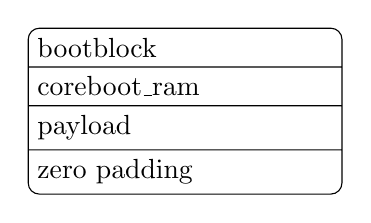
\begin{tikzpicture}
      \node[rectangle split,rectangle split parts=4,draw
           ,text width=3.75cm,rounded corners] (struct) {
        bootblock \nodepart{two}
        coreboot\_ram \nodepart{three}
        payload \nodepart{four}
        zero padding
      };
    \end{tikzpicture}
    \caption{The \emph{coreboot.rom} structure.}
    \label{fig:coreboot.rom}
  \end{center}
\end{figure}

%% .. %%
\subsection{Bootblock}

The \emph{bootblock} is the earliest initialisation code. It's function is
rudimentary, handling only the \emph{reset vector} and enough to \emph{jump} to
the \emph{ROMstage}. The \emph{bootblock} code contains the first
\emph{instruction fetch} that is a \emph{jump instruction} from $4\mbox{GB}$ to
the initialisation code, then an immediate change to $32-\mbox{bit}$
\emph{protected mode}. Once \emph{protected mode} has been toggled, the
\emph{bootblock} provisions the minimal \emph{north} and \emph{south} bridge
setup required to accomplish a \emph{jump} to the \emph{ROMstage}. The
\emph{jump instruction} and subsequent switch to \emph{protected mode} can be
found in:

\begin{verbatim}
  coreboot/src/cpu/x86/16bit
\end{verbatim}

% From Intel's "64 and IA-32 Architectures Software Developer’s Manual" (doc 253668-021 October 2006), Volume 3A, Section 9.1.4:
%  The first instruction that is fetched and executed following a hardware
%  reset is located at physical address 0xFFFFFFF0. This address is 16 bytes
%  below the processor’s uppermost physical address. The EPROM containing the
%  software-initialization code must be located at this address.

\begin{enumerate}

  \item At \textbf{0xFFFFFFF0}, start execution at \textbf{reset\_vector} from
  \textbf{src/cpu/x86/16bit/reset16.inc}, which simply jumps to
  \textbf{\_start}.

  \item \textbf{\_start} from \textbf{src/cpu/x86/16bit/entry16.inc},
  invalidates the TLBs, sets up a GDT for selector 0x08 (code) and 0x10 (data),
  switches to protected mode, and jumps to \textbf{\_\_protected\_start}
  (setting the CS to the new selector 0x08). The selectors provide full flat
  access to the entire physical memory map.

  \item \textbf{\_\_protected\_start} from
  \textbf{src/cpu/x86/32bit/entry32.inc}, sets all other segment registers to
  the 0x10 selector.

  \item Execution continues with various mainboardinit fragments:
  \begin{itemize}
    \item \textbf{\_\_fpu\_start} from \textbf{cpu/x86/fpu\_enable.inc}.
    \item \textbf{(unlabeled)} from \textbf{cpu/x86/sse\_enable.inc}
    \item Some CPUs enable their on-chip cache to be used temporarily as a
    scratch RAM (stack), e.g. \textbf{cpu/amd/model\_lx/cache\_as\_ram.inc}.
  \end{itemize}

\end{enumerate}

The \emph{bootblock} code is written in C and is built into \emph{stackless}
assembler by a custom toolchain. The custom toolchain \emph{ROMCC} is required
due to the restrictive environment of a cold power-up of the hardware.

%% .. %%
\subsection{ROMstage}

The \emph{ROMstage} contains the early chipset and motherboard initialisation,
Cache As RAM setup, memory initialisation, and decompression code for the
coreboot \emph{RAMstage}. Upon \emph{ROMstage} completetion, \emph{RAMstage} is
executed in system memory.

The final mainboardinit fragment is mainboard-specific, in C, called
\textbf{romstage.c}. For non-cache-as-RAM targets, it is compiled with
\textbf{romcc}. It includes and uses other C-code fragments for:

\begin{enumerate}
  \item Initializing MSRs, MTRRs, APIC.
  \item Setting up the southbridge minimally ("early setup").
  \item Setting up Super I/O serial.
  \item Initializing the console.
  \item Initializing RAM controller and RAM itself.
\end{enumerate}

Execution continues at \textbf{\_\_main} from
\textbf{src/arch/x86/init/crt0\_romcc\_epilogue.inc}, where the non-romcc C
coreboot code is copied (possibly decompressed) to RAM, then the RAM entry
point is jumped to.

%% .. %%
\subsection{RAMstage}

\begin{enumerate}
  \item The RAM entry point is \textbf{\_start} in
  \textbf{src/arch/x86/lib/c\_start.S}, where new descriptor tables are set up,
  the stack and BSS are cleared, the IDT is initialized, and
  \textbf{hardwaremain()} is called (operation is now full 32-bit protected
  mode C program with stack).

  \item \textbf{hardwaremain()} is from \textbf{src/boot/hardwaremain.c}, the
  console is initialized, devices are enumerated and initialized, configured
  and enabled.

  \item The payload is called, either via \textbf{elfboot()} from
  \textbf{boot/elfboot.c}, or \textbf{filo()} from \textbf{boot/filo.c}.
\end{enumerate}

% .. %
\section{Coreboot Development}

%% .. %%
\subsection{Development Tools}

\begin{itemize}
  \item \textbf{Minicom} - terminal emulator
  \item \textbf{SAGE Embedded Development Kit (EDK)} - Eclipse-based integrated
  development environment (IDE).
  \item \textbf{SAGE SmartProbe} - Comprehensive hardware interface for
  controlling and viewing the system under development.
\end{itemize}

%% .. %%
\subsection{Source Development}

The source is located in the following directory:

\begin{verbatim}
  coreboot/src/vendorcode
\end{verbatim}

% XXX: draw up the source tree.
..

%% .. %%
\subsection{Critical Hardware Information}

%%% ... %%%
\subsubsection{SuperIO}

The Super I/O chip is found on the mainboards which is responsible for the
serial ports and so first thing to support. Since serial debugging output from
the mainboard via a \emph{null-modem} cable and \emph{minicom} is critically
important to bringing up other components in the process of the Coreboot port.

Adding support for a new Super I/O chip involves the following:

\begin{enumerate}
  \item Add a directory \textbf{src/superio/vendor/device}.
  \item In that directory, add a file \textbf{device\_early\_serial.c} where
  \emph{device} is the actual part name.
  \item In this file you now declare a function
  \textbf{device\_enable\_serial()} which enables the requested serial port.
\end{enumerate}

The \textbf{device\_early\_serial.c} file is where the serial port on the
mainboard is initialised. The serial output will work even before the RAM is
first initialized, thus is required for debugging the RAM initialization
code in a port.

An example of the \textbf{device\_enable\_serial()} function is given:

\begin{lstlisting}[caption=The \textbf{device\_enable\_serial()} function.]
  static void w83627ehg_enable_serial(device_t dev, unsigned int iobase)
  {
         pnp_enter_ext_func_mode(dev);
         pnp_set_logical_device(dev);
         pnp_set_enable(dev, 0);
         pnp_set_iobase(dev, PNP_IDX_IO0, iobase);
         pnp_set_enable(dev, 1);
         pnp_exit_ext_func_mode(dev);
  }
\end{lstlisting}

Mainboards which have this Super I/O chip, can then call this function in their
\textbf{romstage.c} file. For example:

\begin{lstlisting}[caption=The \textbf{romstage.c} file.]
  #include "superio/winbond/w83627ehg/w83627ehg_early_serial.c"
  [...]
  #define SERIAL_DEV PNP_DEV(0x2e, W83627EHG_SP1)
  [...]
  w83627ehg_enable_dev(SERIAL_DEV, TTYS0_BASE);
  uart_init();
  console_init();
\end{lstlisting}

\begin{rem}
  The Super I/O is usually at config address \emph{0x2e} or \emph{0x4e},
  however is mainboard-dependent and so could be different. A way find out the
  address is by running the \emph{superiotool}.
\end{rem}


%%%%%%%%%%%%%%%%%%%%%%%%%%%%
% Chapter: Getting Further %
%%%%%%%%%%%%%%%%%%%%%%%%%%%%
% !TeX encoding=utf8
% !TeX spellcheck = en-AU
%
% Altera Praxis Pty Ltd. [SEC=Open-Source]
%
% Copyright © 2014 Edward O'Callaghan. All Rights Reserved.
%
%%%%%%%%%%%%%%%%%%%%%%%%%%%%%%%%%%%%%%%%%%%%%%%%%%%%%%%%%%%%%%%%%%%%%%%%%
% This file is licensed under Creative Commons Attribution 2.5 License. %
%%%%%%%%%%%%%%%%%%%%%%%%%%%%%%%%%%%%%%%%%%%%%%%%%%%%%%%%%%%%%%%%%%%%%%%%%

\chapter*{Getting further}

You can reach the Coreboot project using the following communication means.

% .. %
\section{IRC}

You can chat with us on IRC using the Freenode Network by joining the
\mbox{\#coreboot} or \mbox{\#flashrom} channels.

% .. %
\section{Mailing-lists}

You can get access to the mailing-lists at
\url{https://lists.coreboot.com}. To ask questions about the
\mbox{something} development please use the \mbox{something-devel} mailing
list.

% .. %
\section{Website}

The \mbox{coreboot} website is at \url{http://www.coreboot.org} has news and
access to the source repositories.


%%%%%%%%%%%%%%%%%%%%%%
% Section : Appendix %
%%%%%%%%%%%%%%%%%%%%%%
\newpage
\appendix

%%%%%%%%%%%%%%%%%%%%%%
% Section : Glossary %
%%%%%%%%%%%%%%%%%%%%%%
\newpage
\printglossaries

%%%%%%%%%%%%%%%%%%%%%%%%%%
% Section : Bibliography %
%%%%%%%%%%%%%%%%%%%%%%%%%%
\newpage
\printbibliography

%%%%%%%%%%%%%%%%%%%
% End of Document %
%%%%%%%%%%%%%%%%%%%
\end{document}
